\documentclass[11pt]{article}
    \usepackage{comment} % enables the use of multi-line comments (\ifx \fi) 
    \usepackage{lipsum} %This package just generates Lorem Ipsum filler text. 
    \usepackage{fullpage} % changes the margin
    % Used for importing figures
    \usepackage{graphicx}
    \usepackage{wrapfig}
    \usepackage{float}
    \usepackage{subcaption}
    
\begin{document}

%Header-Make sure you update this information!!!!
\noindent
\large\textbf{Lab 5} \hfill \textbf{Zach Colbert} \\
\normalsize PH 411 \hfill 21 November 2017\\

\section{Transistor Basics}
\subsection{Introduction}

Transistors are active elements--they control current by means of a "base" signal, separate from the main signal passing through. Junctions between semiconductors make this possible, where electron-hole pairs come together to form a charge imbalance called the "depletion zone," effectively a barrier which prevents electrons from flowing across the junction.\\

By applying some current to the base of the transistor, connected to the middle semiconductor, we suppress the depletion zones enough to open a kind of channel for current to flow through.\\

In addition to acting as electronic switches, starting and stopping current with a small base signal, transistors come with some current gain--by which the input signal is amplified with a still small base singal.\\

In part 1 of this lab, we examine this current gain property of an npn transistor, by two different methods.\\

\subsection{Experimental}

\begin{figure}[H]
    \centering
    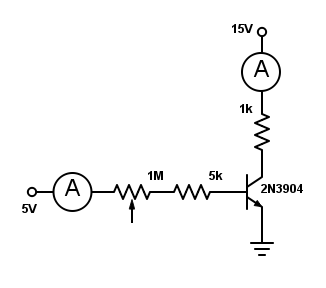
\includegraphics[scale=0.4]{Diagrams/c-1c.png}
    \caption{Simple circuit with an npn transitor.}
    \label{circuit:1c}
\end{figure} 

For this part of the lab, we used a 2N3904 npn transistor. Before looking at the current gain, we used a digital multimeter on the diode setting to show that a transistor behaves like two diodes. We were able to measure voltage drops across the "diodes" on either side of the transistor (base-emitter and collector-base drops) as well as the drop across the entire transistor (collector-emitter drop).\\

Next, as a point of comparison for our current gain, we used the DMM on the transistor gain setting to measure our transistor on its own.\\

Finally, for a little more comprehensive look at the behavior of the transistor over a range of currents, we built the transistor into a circuit and measured the base and collector currents individually.\\

In the above circuit, we used a $1\ M \Omega$ potentiometer to manually adjust the base current, and compared that to the collector current over many samples (keeping the respective input voltages at the collector and base constant throughout). Our theoretical model for the current gain says:

\begin{equation}
I_c = \beta I_b
\end{equation} 

So, we expect a plot of $I_c$ versus $I_b$ to be a line with slope $\beta$, where $\beta$ is the current gain of the transistor.\\

\subsection{Results}

In measuring the "diode" drop voltages across parts of the transistor, we found the following: \\

\begin{center}
    \begin{tabular}[H]{ | l | c | }
        \hline
        Base-Emitter & $0.665\ V$ \\ \hline
        Collector-Base & $0.646\ V$ \\ \hline
        Emitter-Collector & $0\ V$ \\ \hline
    \end{tabular}
\end{center}

The first two measurements showed us that current flows one way through each side of the transistor, just like current flows one way through a diode. The third showed the current-controlling function of the transistor--without a base current, no current flows between the collector and emitter.\\

\begin{figure}[H]
    \centering
    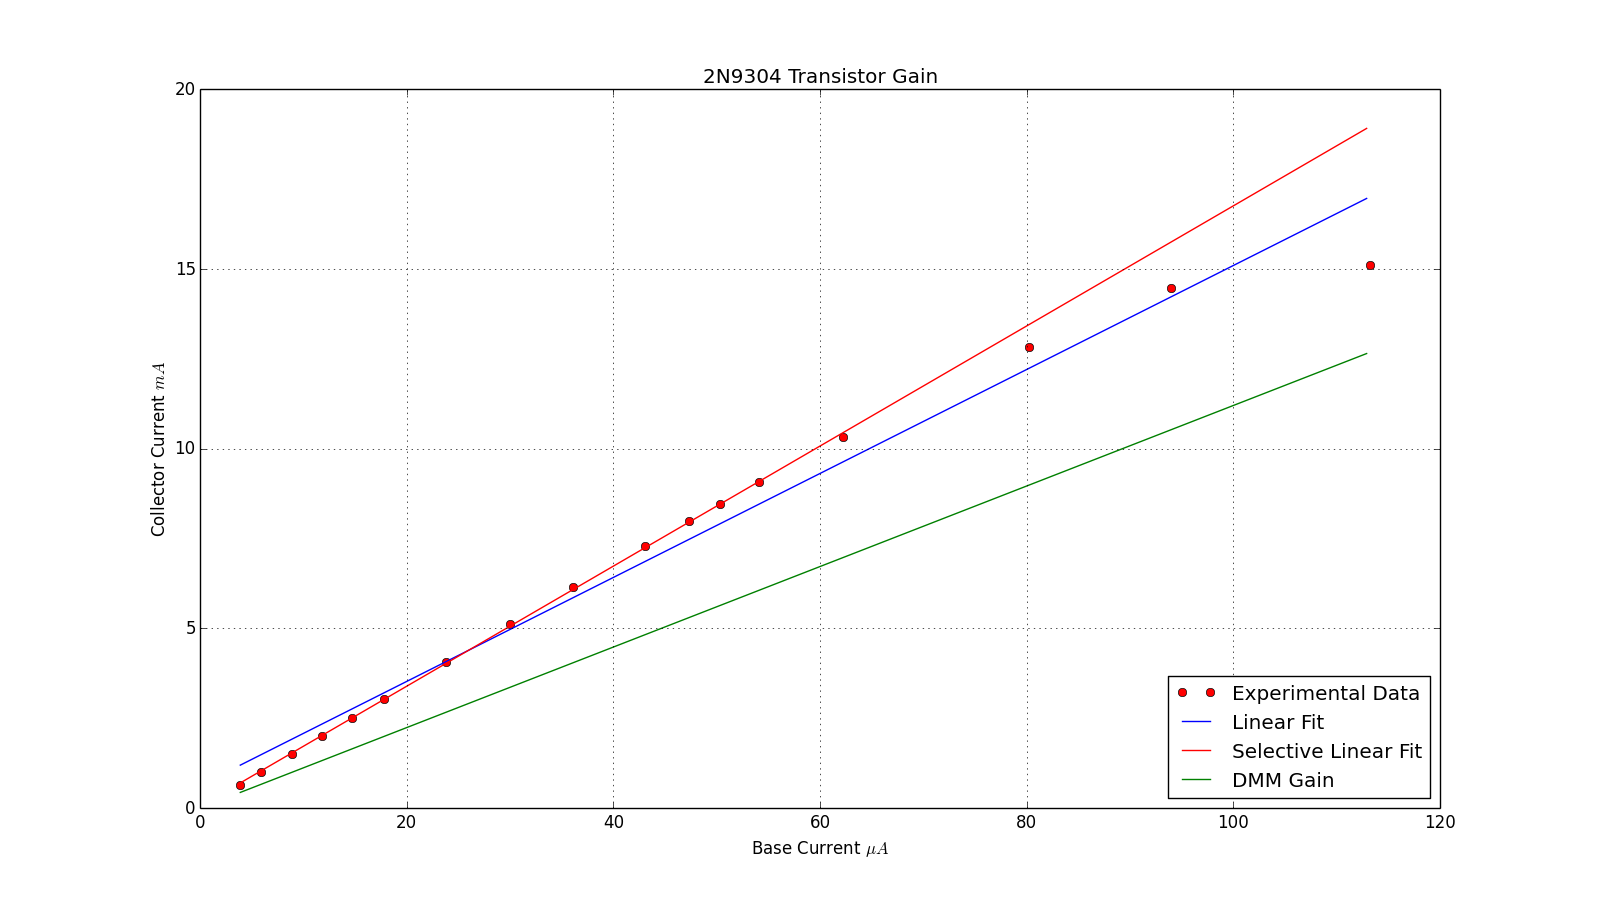
\includegraphics[scale=0.4]{Plots/fig1.png}
    \caption{Current gain of an npn transistor, measured via various methods.}
    \label{fig:1}
\end{figure}

With the DMM on transistor mode, we measured a current gain $\beta = 112$, shown in green on Figure \ref{fig:1}.\\

Our manually measured gain was incredibly consistent, following a distinct line until about $60\ \mu A$ base current. At that point it curved away and became shallow--By some simple analysis of the circuit, this appears to be a maximum for the collector current. \\

That final point lies at about $15\ mA$ collector current. Through a $1\ k \Omega$ resistor, that current results in a $15\ V$ drop between the constant collector voltage $V_{cc}$ and the collector. Not only is that the maximum voltage that can be passed to the collector, it causes the collector voltage to be 0, equal to the emitter voltage. This breaks one of the fundamental rules for normal operation of a transistor.\\

I added a couple of different linear fits to the plot--the line in blue represents a linear fit across all of the data. The line in red represents a linear fit across a select range of data, excluding the points above $60\ \mu A$ base current.\\

The inclusive linear fit represents a current gain of 144, and the exclusive linear fit represents a current gain of 167. I haven't found a good explanation for the difference between these values and the one measured by the DMM initially, but they seem to be reasonably close to each other (at least, within an order of magnitude).\\

\subsection{Conclusion}

There are clear differences between the values measured for current gain in this part of the lab, but it seems reasonable to assume that measurements exclusively made by the DMM are not the most accurate.\\

In this case, if I wanted to characterize this transistor for a larger project, I would tend to choose the current gain found by making a linear fit in the region where the data appears to be linear. Then, at least it is clear what the current gain is for that region, and my larger circuit can be constrained to fit the parameters for normal operation of the transistor.\\
    
%%% PART 2 %%%

\section{Emitter-Follower}
\subsection{Introduction}

In the second part of this lab, we used an emitter-follower circuit to examine the bias of our transistor, and how that affects a given input signal. We also used a couple of more complicated circuits to look at different kinds of signal "clipping" that can happen, and the limiting factors that lead to that clipping.\\

Bias in a transistor is the current or voltage necessary for the transistor to operate normally--that is, for the transistor to perform consistently as a switch or current-limiting device. In this case we focused on the base bias, a voltage applied to the base of the transistor that induces current flow between the collector and emitter.\\

Signal clipping took on a few different forms in this lab. For one circuit, all the negative portions of the signal were completely suppressed. For another, peaks and troughs in the signal appeared to be trimmed from the middle, with a flat region mid-way up a wave. We'll examine these waveforms more closely in the Results section.\\

\subsection{Experimental}

With the emitter-follower circuit, our input and output signals were connected to a common ground. We used a sine wave input, and slowly increased the amplitude of the input signal until we could measure an output signal with an oscilloscope. This minimum input voltage is called the forward bias.\\

Using the math functions on the oscilloscope, we found a waveform representing the difference between the input and output signals to illustrate the signal clipping in a qualitative way.\\

\begin{figure}[H]
    \centering
    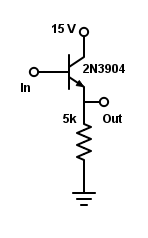
\includegraphics[scale=0.6]{Diagrams/c-2.png}
    \caption{Simple emitter-follower circuit, with the same npn transistor used in part 1.}
    \label{circuit:2}
\end{figure}

With our more complicated circuits, we looked for some limiting factors that lead to signal clipping. For either circuit, we did a lot of work with an oscilloscope probe to find voltage drop across individual elements, but ultimately found our best results by changing the emitter voltage and examining the resultant waveforms.\\

\begin{figure}[H]
    \centering
    \begin{subfigure}{0.4\textwidth}
        \centering
        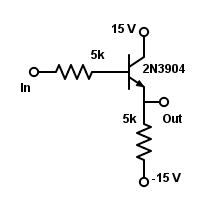
\includegraphics[scale=0.6]{Diagrams/c-2bL.png}
        \caption{Similar to the simple emitter-follower circuit above, with an additional resistor on the transistor base and a constant emitter-side voltage of $-15\ V$ instead of a grounded emitter.}
        \label{circuit:2bL}
    \end{subfigure}
    %
    \begin{subfigure}{0.4\textwidth}
        \centering
        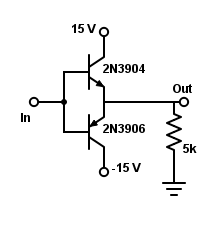
\includegraphics[scale=0.6]{Diagrams/c-2bR.png}
        \caption{A little more complex circuit, which includes a pnp transistor connected emitter-to-emitter with the npn transistor from previous circuits.}
        \label{circuit:2bR}
    \end{subfigure}
\end{figure}

No new theory applies to this part of the lab. Our observations mostly relied on simple Kirchoff analysis of circuits.\\

\subsection{Results}

For the emitter-follower circuit, we found that our input signal had to have a peak-to-peak voltage of at least $700\ mV$. Below that amplitude, there was no measurable output signal.\\

The math function of the oscilloscope was particularly useful for showing the difference between the input and output signals. We were able to see, as we increased the amplitude of the input signal, that the output signal is always clipped at the same amplitude, around $700\ mV$.\\

\begin{figure}[H]
    \centering
    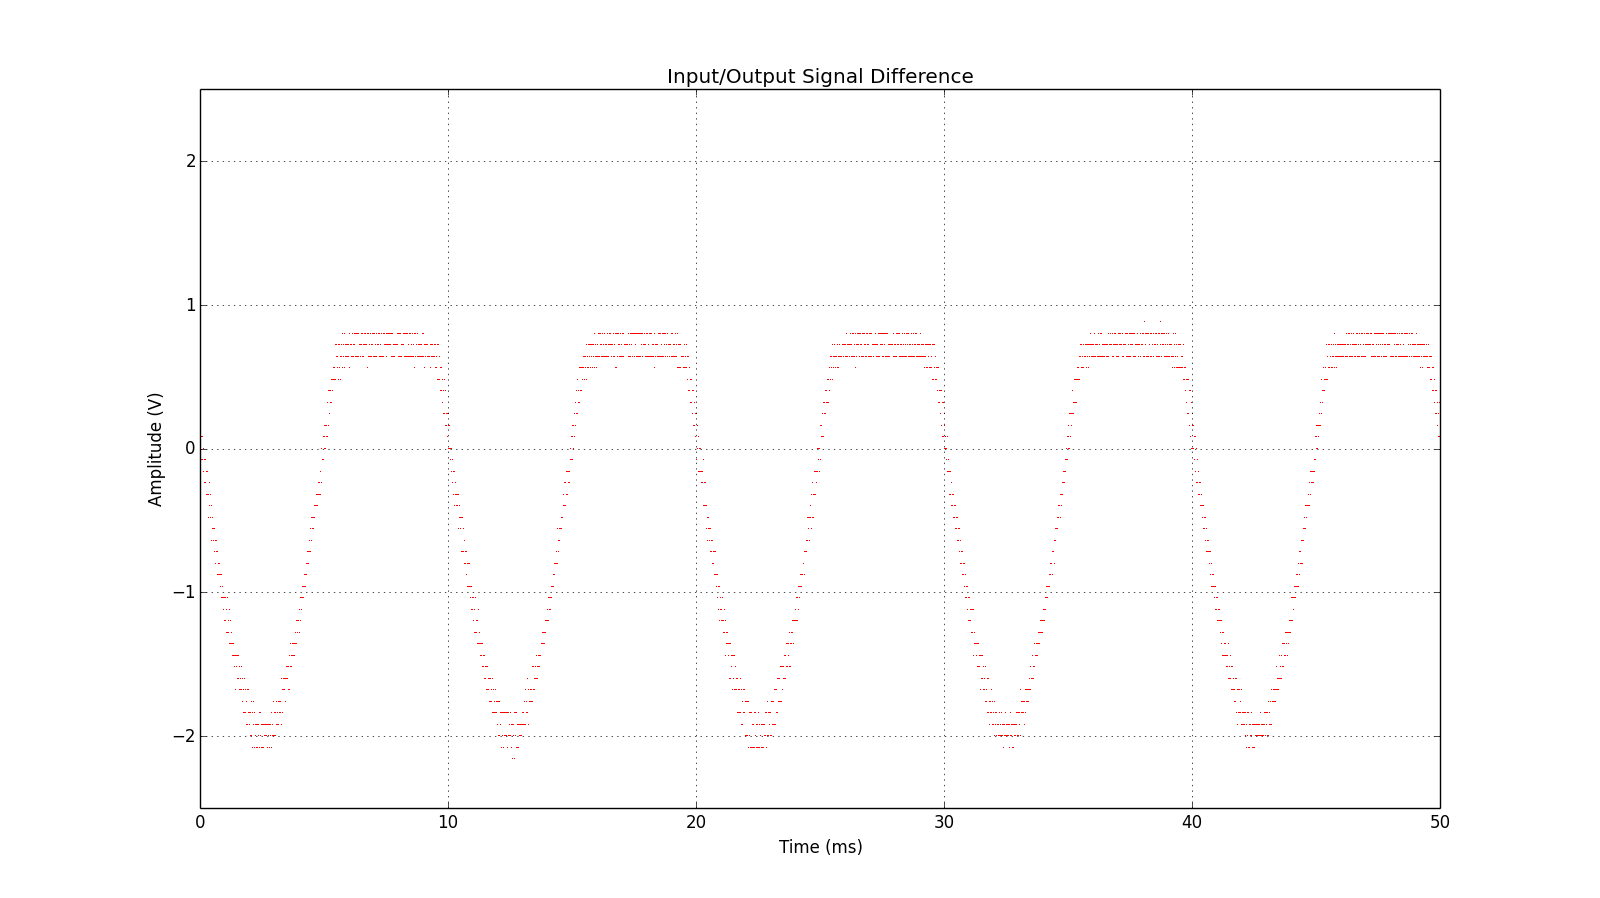
\includegraphics[scale=0.4]{Plots/fig2a.png}
    \caption{The difference between the output and input signals for the simple emitter-follower circuit. This waveform was taken from the math (difference) function of our oscilloscope.}
    \label{fig:2a}
\end{figure}

Using circuit \ref{circuit:2bL} our output signal looked exactly like the input signal, shifted down about $600\ mV$ (voltage offset). With a scope probe we found that the output signal was offset like this after crossing the $5\ k \Omega$ resistor on the transistor base. We also found that by changing the $-15\ V$ near the transistor emitter to ground, the output signal was clipped similar to circuit \ref{circuit:2}.\\

Circuit \ref{circuit:2bR} had an interesting effect on the input signal. Peaks and troughs of the wave were clipped to about $700\ mV$, but clipped from the middle of the wave (about zero volts) instead of from the maxima.\\

\begin{figure}[H]
    \centering
    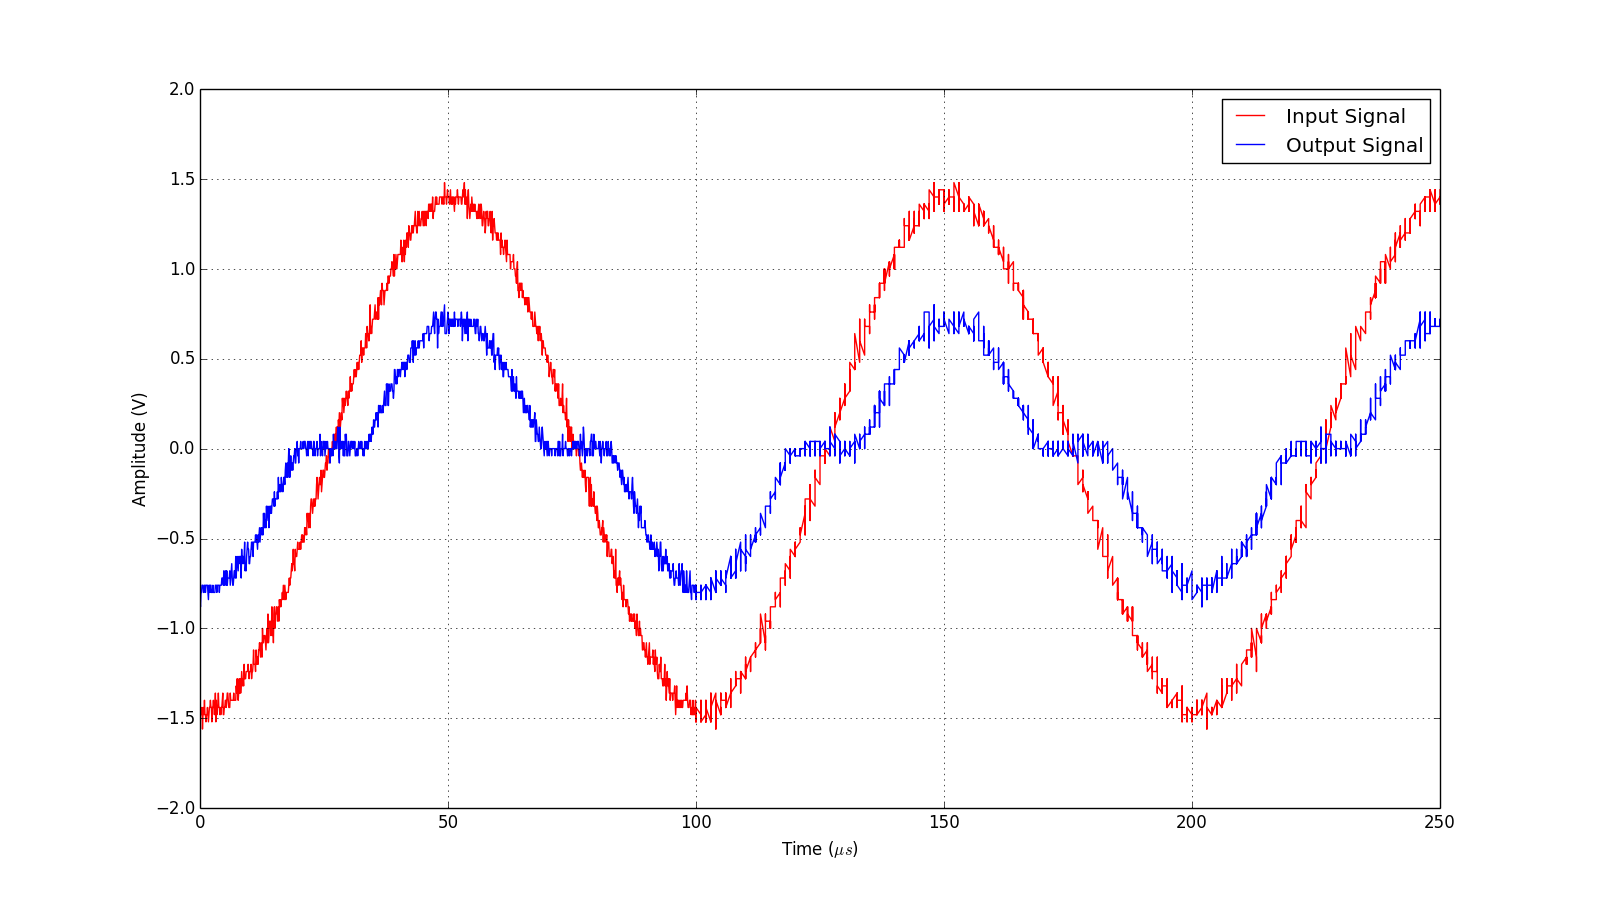
\includegraphics[scale=0.4]{Plots/fig2b.png}
    \caption{The final circuit for part 2 showed some interesting effects--the combination of clipping by the npn and pnp transistors, respectively.}
    \label{fig:2b}
\end{figure}

This shows that the emitter and collector voltages affect the way a signal is clipped when passing through a transistor. Specifically, it appears that npn transistors clip negative regions of the signal where the emitter voltage is zero, and pnp resistors clip positive regions under the same conditions. The combination of these effects is the wave shown in figure \ref{fig:2b}.\\

\subsection{Conclusion}

While it's clear up to this point that transistors are very useful as current-limiting devices and electronic switches, it's now clear that the voltages surrounding a transistor play significant roles in how a signal passing through the device is changed.\\

The clipping effects we observed throughout this part of the lab were very consistent, including the $700\ mV$ value that signals were clipped to. I have not yet been able to use that value to relate the clipped signals to the forward bias of the transistor, but suspect there is some relationship there.\\

%%% PART 3 %%%

\section{Transistor Switch}
\subsection{Introduction}

In the third part of the lab, we simply add a light-emitting diode to our simple transistor circuit to show how the transistor can be used as an electronic switch. The LED enabled us to see visually when current was flowing through the circuit, and when it was not.\\

\subsection{Experimental}

The transistor acts as a switch because of it's forward bias--the threshold where the base voltage is high enough to allow current to flow from the collector to the emitter. This ties back into the concept of the depletion layer, and how it takes a certain voltage to open up a channel for current to flow across the p-n junctions inside the transistor.\\

\begin{figure}[H]
    \centering
    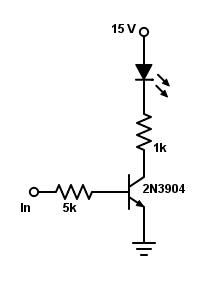
\includegraphics[scale=0.4]{Diagrams/c-3.png}
    \caption{The circuit for part 3 includes the same npn transistor as in part 1. It also uses an LED as a visual cue for current flow through the collector.}
    \label{circuit:3}
\end{figure}

Using the circuit above, we recorded the peak-to-peak input voltage at which the LED started to emit light for a range of frequencies. These measurements gives a general impression of the forward bias of the transistor over that range of frequencies.\\

\subsection{Results}

\begin{center}
    \begin{tabular}[H]{ | l | c | }
        \hline
        Input Frequency (Hz) & Forward Bias (mV) \\ \hline
        10 & 600 \\ \hline
        100 & 600 \\ \hline
        1 k & 600 \\ \hline
        100 k & 600 \\ \hline
        1 M & 700 \\ \hline
        10 M & 2200 \\ \hline
        12.5 M & 2900 \\ \hline
    \end{tabular}
\end{center}

We found that at frequencies higher than $1\ M \Omega$, the forward bias increased dramatically. I suspect that the transistor has a kind of  characteristic time, similar to that of capacitors and inductors--at sufficiently high frequencies, the transistor does not have time to "switch on" before it's bias changes and it is forced to "switch off" again.\\

As a result, very high frequencies require very high biases in order to activate the transistor and allow current to flow.\\

\subsection{Conclusion}

While I'm not positive about my explanation of why the transistor's bias increases dramatically at very high frequencies, it's clear that this could have a significant impact on a circuit containing transistors.\\

In general, it seems safe to assume that the forward bias of a transistor is not necessarily constant with frequency.\\


\end{document}
